\documentclass{article}
\usepackage{textcomp}
\usepackage{tikz}

\newcommand{\crel}{
	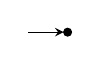
\begin{tikzpicture}[baseline={([yshift=-.8ex]current bounding box.center)}]
		\draw [->, >=stealth] (0,0) -- (0.45,0); 
		\draw [fill] (0.5,0) circle (0.05);
	\end{tikzpicture}
}

\newcommand{\rrel}{
	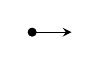
\begin{tikzpicture}[baseline={([yshift=-.8ex]current bounding box.center)}]
		\draw [fill] (0,0) circle (0.05);
		\draw [->, >=stealth] (0.05,0) -- (0.5,0);
	\end{tikzpicture}
}

\newcommand{\mrel}{
	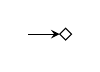
\begin{tikzpicture}[baseline={([yshift=-.8ex]current bounding box.center)}]
		\draw [->, >=stealth] (0,0) -- (0.4,0);
		\draw (0.4,0) -- (0.475,0.075) -- (0.55,0) -- (0.475,-0.075) -- cycle;
	\end{tikzpicture}
}

\newcommand{\irel}{
	\begin{tikzpicture}[baseline={([yshift=-.8ex]current bounding box.center)}]
		\draw [->, >=stealth] (0,0) -- (0.4,0);
		\draw (0.41,0) -- (0.55,0);
		\draw (0.48,-0.07) -- (0.48, 0.07); 
	\end{tikzpicture}
}

\newcommand{\erel}{
	\begin{tikzpicture}[baseline={([yshift=-.8ex]current bounding box.center)}]
		\draw [->, >=stealth] (0,0) -- (0.4,0);
		\draw (0.41,0) -- (0.55,0);
		\draw (0.48, 0.05) circle (0.02);
		\draw (0.48, -0.05) circle (0.02); 
	\end{tikzpicture}
}


\title{DCR/TEE}
\author{Mikkel Gaub \and Malthe Ettrup Kirkbro \and Mads Frederik Madsen}

\begin{document}

\maketitle

\newpage

\tableofcontents

\newpage

\section{Problem}
	The system should support running a distributed DCR graph between multiple parties, under the assumption that any number of those parties will attempt to forge, collude, perjure or otherwise act maliciously, i. e. exhibiting byzantine failures.
	These distributed DCR graphs should always be accessible by all parties, connectivity permitting, and transparency must be ensured for all parties, in that they should always be aware of whether or not activities controlled by that party can be executed at any given time.

	% 1. There must be a happened-before relationship between the execution of an activity and the executions of its dependent activities % Studer Lamports FSM
	% 2. All serializations of the happened-before relationships must be valid execution sequences in DCR % Og opnå enighed om dem

	\section{Definitions}
	\noindent
	Workflow: $G=(V,E)$ \\
	Activities: $V=\{v_1,\ \dots, v_n\}$ \\
	Activity States: $S=\{s_1,\ \dots, s_n\}$, where $s_i \subseteq \{Executed, Pending, Included\}$ corresponding to $V_i$.\\
	Relation: $R=($condition, response, milestone, include, exclude$)$, $e=(v_x, v_y, r_i)$, $E=\{e_1,\ \dots, e_m\}$\\
	Processes: $P =\{p_1,\ \dots, p_o\}$.\\
	History, $H_p(t)$: Sequence of activity executions up to, and at time $t$, as perceived by given process.\\
	Execution: $(v_i, t, p)$, where $v_i$ is the activity executed at time $t$, executed by process $p$.\\
	Dependant activities: An activity, $v_1$ is said to be dependant on another activity, $v_2$, when the DCR rules allowing $v_1$ to be executed, depends on the state of $v_2$. \\
	% Processor: $C$ is said to own a number of specific processes. Any process can only be owned by a single processor. \\
	% Activity responsibility: ... \\

	\section{Requirements}
	\begin{description}
		\item[Consensus]:
			\begin{description}
				\item[Termination] Eventually each correct process sets its decision value (single activity state)
				\item[Partial agreement] % Decision vector = activity state
								Bottom is allowed as substitute for any activity state, unless that activity is owned by process or dependant on one such process. % Hvad er agreement
				\item[Integrity] If $p_i$ is correct, then all correct processes decide on $v_i$, or $\bot$ as the ith component of their vector. % Omformuler. Kan ikke genbruge i på den her måde
			\end{description}
		% \item[Concurrency]: DCR-rules for concurrency (only independent activities can be concurrent) (Tie-breaking). Nødvendig? Argumenter hvorfor Agreement + integrity giver concurrency løsning
		\item[Correctness]: Any state transition must be permitted by DCR logic or they will be rejected by correct nodes.
		\item[Non-repudiation]: $v_i$ must be provably proposed by $p_i$, within the bounds specified by any applied cryptography.
		% \item[Co-non-repudiation?]:
	\end{description}

	\section{Scenarios} % Omformuleres til at bruge definitions.
	\begin{description}
		\item[Scenario 1]
			$A\crel B$\\
			Alice must never decide $\bot$ for $A$. Bob must never decide $\bot$ for either $A$ or $B$.
		\item[Scenario 2]
			$A\crel B$, $A\crel C$\\
			Alice, Bob and Charlie must always decide the same value for $A$.\\
			Problem: Prevent Alice from telling Bob the state, but not Charlie. (Reduces to FLP.)
		\item[Scenario 3]
			$A\erel B$, $B\crel C$\\
			Alice and Bob must agree on the state of $A$, Bob and Charlie must agree on the state of $B$, only Charlie must agree on the value of $C$.
		\item[Scenario 4]
			$A\erel B$, $B\erel A$\\
			Both Alice and Bob must agree on both $A$ and $B$.\\
			Problem: Concurrency.
		\item[Scenario 5]
			$A\irel C$, $A\irel D$, $B\erel C$, $B\erel D$\\
			Both Alice and Bob must agree on only $A$ and $B$, respectively. Charlie must agree on everything except $D$, and Dahlia must agree on everything except $C$\\
			Problem: Concurrency (expanded), not serially equivalent if $C$ is included and $D$ is excluded after $A$ and $B$ have executed concurrently.
	\end{description}

	\section{Locking}

	\begin{description}
		\item[1: Exclude-include] $A \erel D, A \irel C, B \erel C, B \irel D$
		\item[2: Include condition] $A \irel C, C \crel B, B \irel D, D \crel A$ where $C$ and $D$ are excluded.
		\item[3: Non-modifying to condition] $A \irel C, C \crel B, B \irel D, D \crel A, E \erel C$ where $D$ is excluded.
	\end{description}

	\noindent There are three ways of locking when executing:

	\begin{description}
		\item[2 degrees back] has the disadvantage that notifications have to be pushed independently of locking. This locking does not work for graph 1, as A and B do not need to acquire locks on C and D. This means that the end state is subject to race conditions.
		\item[All adjacent] notifications need to be pushed in the second degree ocasionally (graph 2).
		\item[2 degrees forward] has the inherent advantage of notifying relevant activities on execution. In graph 3, an execution of $A$ would only require locking on C, as opposed to the \emph{All adjacent locking} scheme, which would require that D should be locked as well.
	\end{description}

	It seems that, given the state of all relevant nodes, the locking mechanism described as \emph{2 degrees forward} minimizes the amount of locks needed for any execution.
	This optimization is, however, only possible when the state of $C$ is known and since locking is only performed forwards, there is no implicit way to propogate executions backwards.
	This means that $A$ does not know the state of $C$ on execution and would have to do one of two options when executing:
	\begin{itemize}
		\item $A$ sends a locking message to $C$, telling it to lock $B$ if necessary.
		\item $A$ sends a locking message to $C$ and one to $B$, but gives $B$ the option to forego locking if the state of $C$ would be unchanged by the execution of $A$.
	\end{itemize}
	Both options result in the minimum amount of locks, but the first option has fewer messages, as it only results in two messages.
	However, the first option has the disadvantage of potentially taking twice as long, assuming that transporting a message between $A$ and $C$ takes the same amount of time as between $A$ and $B$.

	% trade-off besked vs. låse vs. round-trips

	\section{The algorithm}
	Consider the activities $A$, $B$ and $C$, where $A$ has relation $AB$ to $B$, and $B$ has relation $BC$ to $C$.
	We will describe the algorithm under the maximally distributed case where each activity is handled by a separate peer.
	For simplicity i.e. $A$ will refer to both the activity and the peer responsible for it.
	% We will show that this workflow is enough to describe a general algorithm when $A$ is executed.

	% Effects must push execution state
	When $AB$ is an effect ($A\irel B$, $A\erel B$, $A\rrel B$), $B$ must be informed of any execution of $A$.
	To see this is the case, consider the workflow $(\{D, E, F\}, \{D\erel F, E\irel F\})$.
	As $F$ is not immediately informed about executions of $D$ and $E$, an execution attempt at $F$ must query $D$ and $E$ to determine the inclusion state of $F$.
	Such a query would require an ordering of executions of $D$ and $E$, which is not generally possible in an asynchronous setting.

	% AB effects must synchronize
	Further, when $AB$ is an effect, some degree of synchronization must occur between a subset of peers.
	To see this is the case, consider the workflow $(\{D, D', E, E'\}, \{D\irel E, D\erel E', D'\erel E, D'\irel E\})$.
	We showed executions must be propagated along effects in an asynchronous setting.
	Thus when executing $D$ and $D'$, messages $M_{D\irel E}$, $M_{D\erel E'}$, $M_{D'\erel E}$ and $M_{D'\irel E'}$ are required.
	The ordering of these messages can not generally be guaranteed in an asynchronous setting.
	To see why synchronization must occur, consider the message arrival sequence $(M_{D\irel E}, M_{D'\erel E}, M_{D'\irel E'}, M_{D\erel E'})$, resulting in an invalid workflow state where both $E$ and $E'$ are excluded.

	% Execute A, lock B
	% Execute B, lock A

	% AB effects, BC constaints must synchronize
	When $AB$ is an effect and $BC$ is a constraint ($B\crel C, B\mrel C$),

	% Forward locking
	% Backward locking
	% Foward-backward locking

	When $A$ is executed:\\
	$B$ must be locked if:\\
	$AB$ is an effect (include, exclude, response)\\
	$C$ must be locked if:\\
	$AB$ is a constraining effect, and $BC$ is a constraint (condition, milestone), in the following configuration:\\
	\begin{itemize}
		\item $A \irel B \crel C$ (B is excluded)
		\item $A \irel B \mrel C$ (B is excluded and pending)
		\item $A \rrel B \mrel C$ (B is not pending)
	\end{itemize}

	\section{Consensus}:\\
	N processes: $p_1, p_2 \dots, p_n$\\
	N proposed values: $\{v_1, v_2 \dots, v_n\}$, where each $v$ is a value from unspecified set $D$.
	N decision variables: $\{d_1, d_2, \dots, d_n\}$
	Process $p_i$ moves from \textit{undecided} state to \textit{decided} by proposing $v_i$ and setting $d_i$ s.t:\\
	\begin{description}
		\item[Termination]: Eventually each correct process sets its decision variable.
		\item[Agreement]: The decision value of all correct processes is the same.
		\item[Integrity]: If the correct processes all proposed the same value, then any correct process in the decided state has chosen that value.
	\end{description}
	
	\noindent
	\subsection{Distributed DCR (D-DCR)}:\\
	Given the distributed DCR-graph $G$.
	\begin{description}
		\item[Consensus]:
			\begin{description}
				\item[Termination] Eventually each correct process sets its decision value (single activity state)
				\item[Agreement] Decision vector = activity states
								1. Eventual agreement: We can poll for an history, after which agreement on current state is reached.
								2. Partial agreement: Bottom is allowed as substitute for any activity state (not if you're responsible for that activity)
				\item[Integrity] If $p_i$ is correct, then all correct processes decide on $v_i$, or $\bot$ as the ith component of their vector.
			\end{description}
		\item[Concurrency]: DCR-rules for concurrency (only independent activities can be concurrent) (Tie-breaking)
		\item[Correctness]: For a correct peer to propose a changed activity state, the new activity state must be the result of a valid activity execution in the last decided decision vector. We assume an agreed upon genesis state.
		\item[Non-repudiation]: $v_i$ must be provably proposed by $p_i$, within a negligible probability.
		% \item[Co-non-repudiation?]:
	\end{description}

	\noindent
	\subsection{Reduction from D-DCR to consensus (no concurrency)}:\\
	(Assume initial state is agreed upon)\\
	Let $D$ be the set of possible decision vectors.\\
	Any correct process will only choose a decision vector that is obtainable by executing an activity that is in an executable state in the last agreed upon decision vector. (Correctness)\\
	% The decision vector must be proposed by an actor with execution rights of the 
	Use consensus to decide on a possible execution.\\

	\noindent
	\subsection{Reduction from consensus to D-DCR}:\\
	For each $v$ in $D$ create an activity $a$ in a DCR-graph.\\
	Let all activities exclude all other activities (no concurrency).\\
	All actors can execute all activities.
	When a peer chooses a $v_i$, model this as trying to execute the corresponding $a_i$.
	Run D-DCR.\\
	When an execution is completed, set $d_i$ as the $v_i$ corresponding to the executed activity.

		

\end{document}